\documentclass{article}
\usepackage[utf8]{inputenc}
\usepackage[left=1in,right=1in,top=1in,bottom=1in]{geometry}
\usepackage{crop,graphicx,array,color,flushend,stfloats,amsthm,chngpage,times,fancyhdr,lipsum,lastpage}

%%%%%%%%%%%%   Extra libraries & settings %%%%%%%%%%%%%
\setlength{\parskip}{0.25em}

%%%%%%%%%%%%   Header and Footer  %%%%%%%%%%%%%
\pagestyle{fancy}

\fancypagestyle{plain}{%
  \renewcommand{\headrulewidth}{0pt}%
  \fancyhf{}%
  \fancyfoot[R]{Page \bf\thepage\ \rm of \bf\pageref{LastPage}}%
}


%%%% Customise Titles and Headers: %%%%
\title{Don't forget adding title}
\author{Chinchuthakun Worameth (18B00033)}
\date{\today}

\fancyhf{}
\fancyhead[L]{Chinchuthakun Worameth}
\fancyhead[R]{18B00033}
\fancyfoot[R]{Page \bf\thepage\ \rm of \bf\pageref{LastPage}}


\AtBeginDocument{
%%%%%%%%%%%% Make Title and Format Lines %%%%%%%%%%%%
\maketitle											%
\vspace{-120px}										%
\noindent\rule{\linewidth}{1pt} \par				%
\vspace{100px}										%
\vspace{-20px}										%
\noindent\rule{\linewidth}{1pt} \par				%
\vspace{10px}										%
% %%%%%%%%%%%%%%%%%%% Content %%%%%%%%%%%%%%%%%%%%	
}

\AtEndDocument{
\bibliographystyle{IEEEtran}
\nocite{*}
\bibliography{citation}
}
% math stuff
\usepackage{amsmath}                % to use DeclareMathOperator
\usepackage{amssymb}
\usepackage{mathrsfs}
\usepackage{mathtools}
\usepackage{xargs}                  % for more than one optional arguments when define new commands
\usepackage{physics}                % vectors
\usepackage{mdframed}               % frames for definition, theorem, etc.
\usepackage[ruled]{algorithm2e}     % for algorithms
\usepackage{ifthen}                % for \ifthenelse
\usepackage{upgreek}

% figures and tables
\usepackage{titlesec}
\usepackage{caption}
\usepackage{subcaption}
\usepackage{multirow}
\usepackage{relsize}

% formatting some important single letters
\renewcommand{\epsilon}{\varepsilon}
\renewcommand{\phi}{\varphi}
\renewcommand{\upepsilon}{\upvarepsilon}
\renewcommand{\upphi}{\upvarphi}

% new operators
\DeclareMathOperator*{\argmin}{arg\,min}                % argmin
\DeclareMathOperator*{\argmax}{arg\,max}                % argmax
\DeclarePairedDelimiter\ceil{\lceil}{\rceil}            % ceiling function
\DeclarePairedDelimiter\floor{\lfloor}{\rfloor}         % floor function
\DeclarePairedDelimiter{\parens}{\lparen}{\rparen}      % parenthesis (use \parens* for automatically adjusting version)
\DeclarePairedDelimiter{\bracket}{[}{]}
\DeclarePairedDelimiter{\cbracket}{\{}{\}}
\DeclarePairedDelimiter{\ang}{\langle}{\rangle}
% \DeclarePairedDelimiter{\fourier}{\mathscr{F}\{}{\}}
% \DeclarePairedDelimiter{\invfourier}{\mathscr{F}^{-1}\{}{\}}

\newcommand{\fourier}[1]{\mathscr{F}\cbracket*{#1}}
\newcommand{\invfourier}[1]{\mathscr{F}^{-1}\cbracket*{#1}}
\newcommand {\dx}{\,dx}
\newcommand {\dy}{\,dy}
\newcommand {\dz}{\,dz}
\newcommand {\dt}{\,dt}
\newcommand {\du}{\,du}
\newcommand {\dtheta}{\,d\theta}
\newcommand {\domega}{\,d\omega}



\newcommand{\bigo}[1]{\ensuremath{\mathcal{O}\parens*{#1}}}
% new commands
\newcommand{\st}{such that }
\newcommand{\w}{where }
\newcommand{\del}{\nabla}
\newcommand{\larrow}{\leftarrow}
\newcommand{\rarrow}{\rightarrow}
\newcommand{\tbf}{\textbf}
\newcommand{\tit}{\textit}
\newcommand{\col}{\operatorname{col}}
\newcommand{\mat}[1]{\begin{matrix} #1 \end{matrix}}
% \newcommand{\vect}[1]{\boldsymbol{\mathbf{#1}}}
\newcommand{\vf}[1]{\boldsymbol{\mathbf{#1}}}
\newcommandx*{\seq}[2][1,2]{\ensuremath{#1, \ldots, #2}}
\newcommandx*{\ssum}[3][1,2,3]{\ensuremath{\sum_{#1 = #2}^{#3}}}
\newcommandx*{\sint}[2][1,2]{\ensuremath{\int_{#1}^{#2}}}
% \newcommandx*{\func}[4][1,2,3,4]{\ensuremath{#1^{\parens{#2}}_{#3}\parens{#4}}}
% \newcommandx*{\val}[3][1,2,3]{\ensuremath{#1^{\parens{#2}}_{#3}}}

% \newcommandx*{\func}[4][1=f,2=x,3,4, usedefault]{
%     \ifthenelse{\equal{#3}{}}{\ensuremath{#1_{#4}\parens{\vf{#2}}}}{\ensuremath{#1^{\parens{#3}}_{#4}\parens{\vf{#2}}}}
% }
\newcommandx*{\func}[3][1=f,2,3, usedefault]{
    \ifthenelse{\equal{#2}{}}{\ensuremath{#1_{#3}}}{\ensuremath{#1^{\parens{#2}}_{#3}}}
}
\newcommandx*{\val}[3][1,2,3, usedefault]{
    \ifthenelse{\equal{#2}{}}{\ensuremath{\vf{#1}_{#3}}}{\ensuremath{\vf{#1}^{\parens{#2}}_{#3}}}
}

\newcommandx*{\Real}[1][1, usedefault]{\ensuremath{\mathbb{R}^{#1}}}                % set of real number
\newcommandx*{\Int}[1][1, usedefault]{\ensuremath{\mathbb{Z}^{#1}}}                 % set of integer
\newcommandx*{\Natural}[1][1, usedefault]{\ensuremath{\mathbb{N}^{#1}}}             % set of natural number
\newcommandx*{\normal}[2][1=0, 2=1, usedefault=!]{\ensuremath{\mathcal{N}(#1,#2)}}  % Gaussian distribution

% define frame environment
% \newmdtheoremenv{definition}{Definition}
% \newmdtheoremenv{proposition}{Proposition}
% \newmdtheoremenv{corollary}{Corollary}
% \newmdtheoremenv{lemma}{Lemma}
% \newmdtheoremenv{theorem}{Theorem}
% \newmdtheoremenv{remark}{Remark}

% define keywords for algorithm
\SetKwInOut{Input}{Input}
\SetKwInOut{Output}{Output}
\SetKwInOut{Parameter}{Parameter}

% \begin{theorem}{text}{label}
% refer as \ref{tha:label}
\usepackage{tcolorbox}
\tcbuselibrary{theorems,breakable} %% を読み込む
\definecolor{burgundy}{rgb}{0.5, 0.0, 0.13}
\newtcbtheorem[number within=section]{theorem}{Theorem}%
{colframe=burgundy,colback=burgundy!2!white,
rightrule=0pt,leftrule=0pt,bottomrule=2pt,
colbacktitle=burgundy,theorem style=standard,breakable,arc=0pt}{theo}

\definecolor{oxfordblue}{rgb}{0.0, 0.13, 0.28}
\newtcbtheorem[number within=section]{definition}{Definition}%
{colframe=oxfordblue,colback=oxfordblue!2!white,
rightrule=0pt,leftrule=0pt,bottomrule=2pt,
colbacktitle=oxfordblue,theorem style=standard,breakable,arc=0pt}{def}

\definecolor{cadmiumorange}{rgb}{0.93, 0.53, 0.18}
\newtcbtheorem[number within=section]{remark}{Remark}%
{colframe=cadmiumorange,colback=cadmiumorange!2!white,
rightrule=0pt,leftrule=0pt,bottomrule=2pt,
colbacktitle=cadmiumorange,theorem style=standard,breakable,arc=0pt}{rem}

% equation numbering
\numberwithin{equation}{section}

%%%%%%%%%%%%%%%%%%%%%%%%%%%
\usepackage{listings}
\usepackage{xcolor}

\definecolor{codegreen}{rgb}{0,0.6,0}
\definecolor{codegray}{rgb}{0.5,0.5,0.5}
\definecolor{codepurple}{rgb}{0.58,0,0.82}
\definecolor{backcolour}{rgb}{0.95,0.95,0.92}

\lstdefinestyle{mystyle}{
    backgroundcolor=\color{backcolour},   
    commentstyle=\color{codegreen},
    keywordstyle=\color{magenta},
    numberstyle=\tiny\color{codegray},
    stringstyle=\color{codepurple},
    basicstyle=\ttfamily\footnotesize,
    breakatwhitespace=false,         
    breaklines=true,                 
    captionpos=b,                    
    keepspaces=true,                 
    numbers=left,                    
    numbersep=5pt,                  
    showspaces=false,                
    showstringspaces=false,
    showtabs=false,                  
    tabsize=2
}

\lstset{style=mystyle}

\makeatletter
\renewcommand*\env@matrix[1][\arraystretch]{%
  \edef\arraystretch{#1}%
  \hskip -\arraycolsep
  \let\@ifnextchar\new@ifnextchar
  \array{*\c@MaxMatrixCols c}}
\makeatother
\usepackage{subfiles}
\usepackage{subcaption}
\usepackage{hyperref}

\title{Computer Graphics Assignment \#5}
\begin{document}
\section{Question}
\begin{enumerate}
    \item The graphs in Figure \ref{assignment5-problem1} are pigment spectral reflectances. Calculate the CIEXYZ1931 coordinate of the reflection of those pigments with D65 incident light. You can assume that the reflectance values at less than 400nm are equal to the value at 400nm and the reflectance values at greater than 700nm are equal to the value at 700nm, and approximate the spectrum of the D65 light as black-body radiation at 6504K. The color matching functions for CIEXYZ1931 shown in Figure \ref{assignment5-problem2} is XYZ\_CIE\_2.dat.
    \item Calculate the color coordinate of the reflection of pigments in sRGB(8bits) color space, where the reflection of a surface, whose reflectance at any wavelength is 100%, with a D65 incident light is (255,255,255).
    \item Answer the numbers of the brightest and darkest pigments in the D65 illumination condition.
\end{enumerate}

\begin{figure}[h]
    \centering
    \hspace*{\fill}
    \subcaptionbox{Pigment Reflectances \label{assignment5-problem1}}{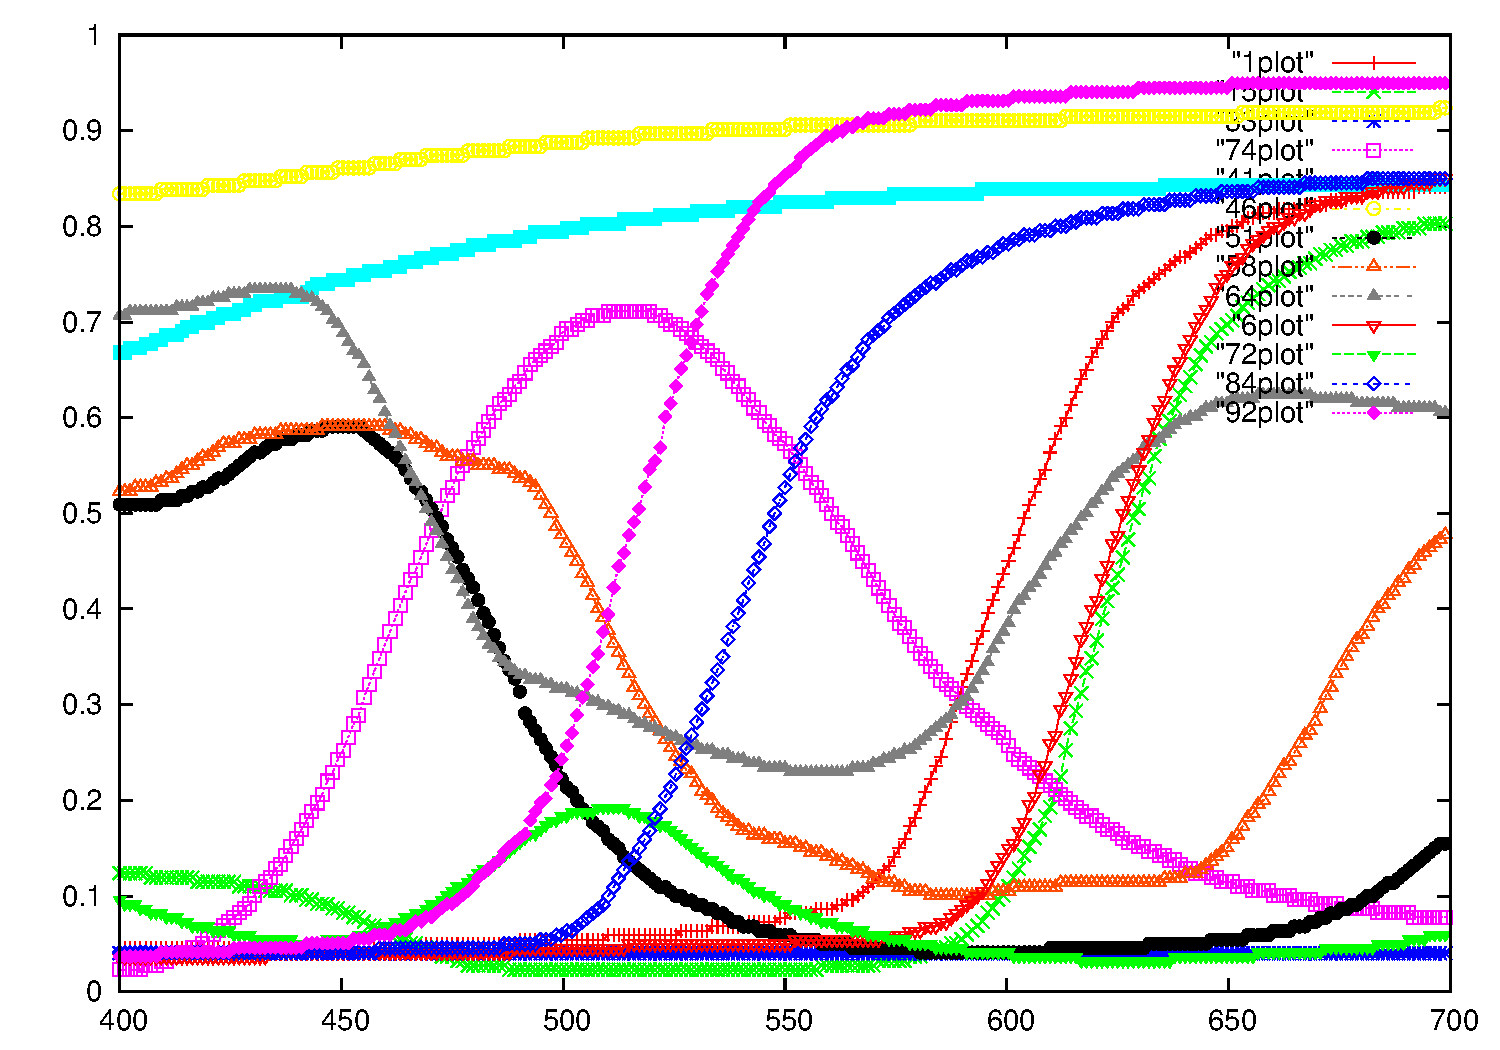
\includegraphics[width=0.45\textwidth]{figures/assignment5/assignment5-problem1.png}}%
    \hspace*{\fill}
    \subcaptionbox{CIEXYZ1931 Standard Observer Color Matching Functions \label{assignment5-problem2}}{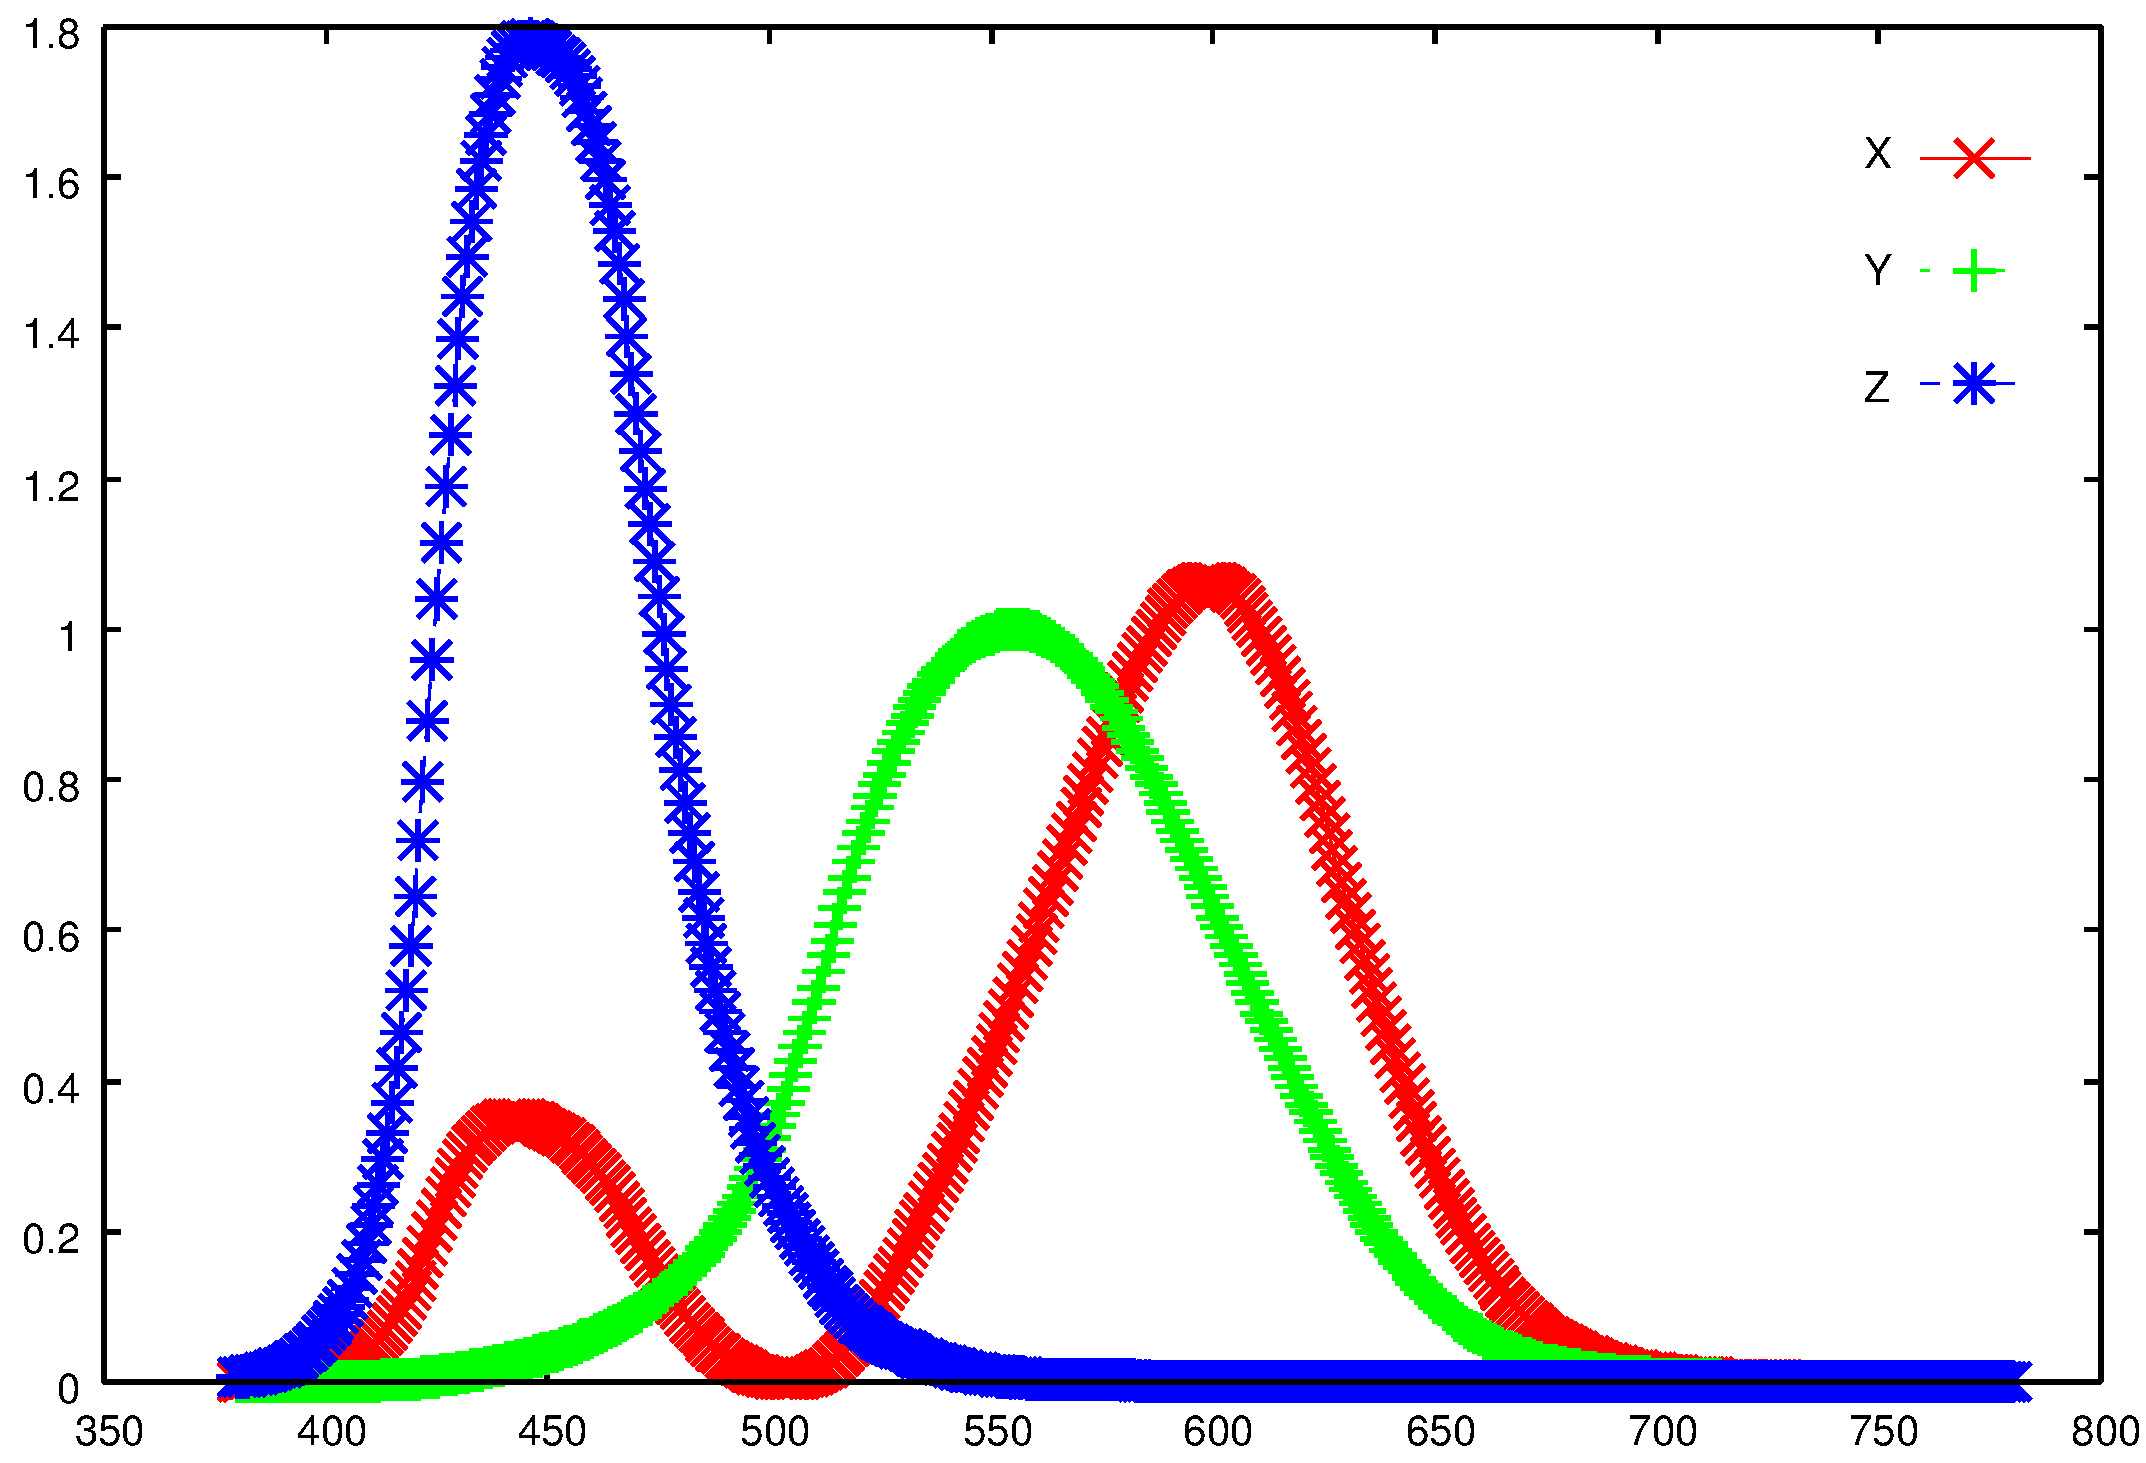
\includegraphics[width=0.5\textwidth]{figures/assignment5/assignment5-problem2.png}}%
    \hspace*{\fill}
    \caption{Given data}
\end{figure}

\section{Answer}

This report describes only procedures and results. Please refer to \href{https://colab.research.google.com/drive/1KD-4itGSez7aZ8Xvt2FDbf4bOZyQURiZ?usp=sharing}{\underline{this Python imeplementation}} for detailed numerical calculations. Although I have already verified that we can access this link, please contact me if you could not access it for some reason when grading this assignment.

\subsection{XYZ Coordinate System}

\subsubsection{General Procedure}
Let $S(\lambda)$ and $I(\lambda)$ denote reflectance of pigment and relative spectral power at wavelength $\lambda$, respectively. We can define reflection at each $\text{Ref}(\lambda)$ as

\begin{equation}
    \text{Ref}(\lambda) = S(\lambda)I(\lambda)
\end{equation}

By using CIEXYZ1931 matching functions, we can calculate the CIEXYZ1931 coordinate of the reflection of those pigments with a D65 incident light as

\begin{subequations}
    \begin{gather}
        X = \frac{1}{N}\int_{380}^{780} \text{Ref}(\lambda) \bar{x}(\lambda) ~d\lambda \approx \frac{1}{N}\sum_{380}^{780} \text{Ref}(\lambda) \bar{x}(\lambda)\\
        Y = \frac{1}{N}\int_{380}^{780} \text{Ref}(\lambda) \bar{y}(\lambda) ~d\lambda \approx \frac{1}{N}\sum_{380}^{780} \text{Ref}(\lambda) \bar{y}(\lambda)\\
        Z = \frac{1}{N}\int_{380}^{780} \text{Ref}(\lambda) \bar{z}(\lambda) ~d\lambda \approx \frac{1}{N}\sum_{380}^{780} \text{Ref}(\lambda) \bar{z}(\lambda)\\
        N = \int_{380}^{780} I(\lambda) \bar{y}(\lambda) ~d\lambda \approx \sum_{380}^{780} I(\lambda) \bar{y}(\lambda)
    \end{gather}
\end{subequations}
where $\bar{x}(\lambda)$, $\bar{y}(\lambda)$, and $\bar{z}(\lambda)$ are the values of matching functions for $X$, $Y$, and $Z$ at wavelength $\lambda$, respectively \cite{assignment5-xyz-wikipedia}. After performing these calculations, XYZ coordinate for each pigment is given in Figure \ref{assignment5-xyz}.

\subsubsection{Implementation Detail}

Although the general procedure is straightforward, reflectance data require some preparation because they are not measured at the same wavelengths as CIEXYZ1931 matching functions. Specifically, we perform the following steps:
\begin{enumerate}
    \item Since a pigment's reflectance is measured at 400 nm, reflectance values at less than 400 nm is equal to the value at 400 nm.
    \item Reflectance values in the range 400 to 700 are approximated as a linear interpolation of two closest values. Note that since the data point with maximum wavelength locates at less than 700 nm, the value at 700 nm is extrapolated.
    \item Following the given instruction, reflectance values at greater than 700 nm are equal to the value at 700 nm. 
\end{enumerate}

Another issue is the lack of relative spectrum power of D65 incident light. Consequently, we will approximate the spectrum of the D65 light as black-body radiation at 6504K, which is given by

\begin{equation}
L_e(\lambda) = \frac{2c^2h}{\lambda^5(e^{hc / kT\lambda} - 1)}
\end{equation}
where $h = 6.6260755 \times 10^{-34}$, $c = 2.99792458 \times 10^8$, $k = 1.380658 \times 10^{-23}$ at $T = 6504$ for $\lambda \in [380,780]$. Note that the illustration for interpolated reflectance values of pigments and relative spectrum power (to wavelength at 560 nm) are shown in Figure \ref{assignment5-pigment} and \ref{assignment5-spectrum}, respectively.

\begin{figure}[h]
    \centering
    \hspace*{\fill}
    \subcaptionbox{Interpolated pigment reflectances \label{assignment5-pigment}}{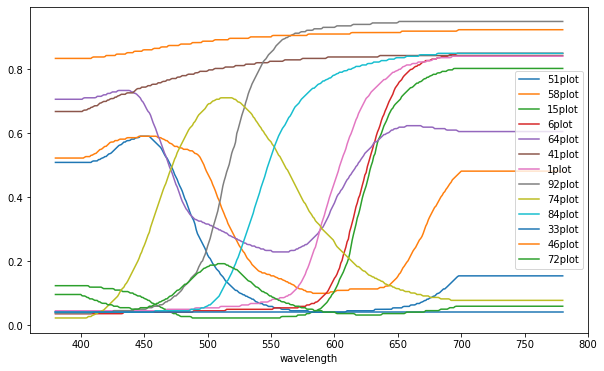
\includegraphics[width=0.45\textwidth]{figures/assignment5/assignment5-pigment.png}}%
    \hspace*{\fill}
    \subcaptionbox{Relative spectrum power (to wavelength at 560 nm) \label{assignment5-spectrum}}{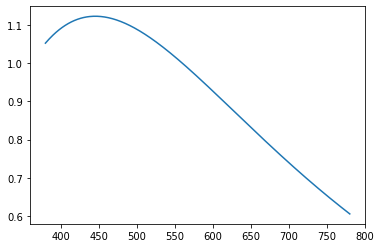
\includegraphics[width=0.45\textwidth]{figures/assignment5/assignment5-spectrum.png}}%
    \hspace*{\fill}
    \caption{Necessary preprocessed data for problem \#1}
\end{figure}

\subsection{sRGB Coordinate System}

\subsubsection{General Procedure}
Given a XYZ coordinate $(X,Y,Z)$, its equivalent color in sRGB system $(R_{8bit}, G_{8bit}, B_{8bit})$ is given by

\begin{equation}
    C_{8bit} = \begin{cases}
    \text{round}\parens*{255(12.92C')} &,~ C' < 0.031308 \\
    \text{round}\parens*{255\parens*{1.055C'^{1.0/2.4} - 0.55}} &,~ \text{otherwise}
    \end{cases}
\end{equation}
where $C' \in \{R', G', B'\}$ and
\begin{equation}
    \begin{pmatrix}
        R' \\
        G' \\
        B' \\
    \end{pmatrix} = 
    \begin{pmatrix}
        3.2406 &    -1.5372 &   -0.4986 \\
        -0.9689 &    1.8758 &   0.0415 \\
        0.0557 &    -0.2040 &   1.0570 \\
    \end{pmatrix}
    \begin{pmatrix}
        X \\
        Y \\
        Z \\
    \end{pmatrix}
\end{equation}
    
We assume that the reflection of a surface, whose reflectance at any wavelength is 100\%, with a D65 incident light is $(255,255,255)$. After performing these calculations, sRGB coordinate for each pigment is given in Figure \ref{assignment5-sRGB}.

\subsubsection{Implementation Detail}
Unlike the previous problem, the XYZ coordinates do not require any specific preprocessing before applying the mathematical relationships described above.

\begin{figure}[h]
    \centering
    \resizebox{0.6\textwidth}{!}{
        \hspace*{\fill}
        \subcaptionbox{XYZ coordinate \label{assignment5-xyz}}{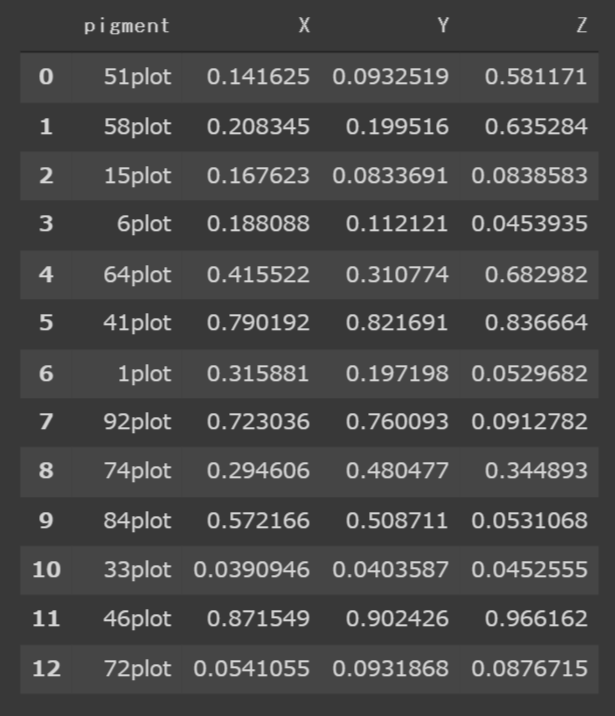
\includegraphics[width=0.56\textwidth]{figures/assignment5/assignment5-xyz.png}}%
        \hspace*{\fill}
        \subcaptionbox{sRGB coordinate \label{assignment5-sRGB}}{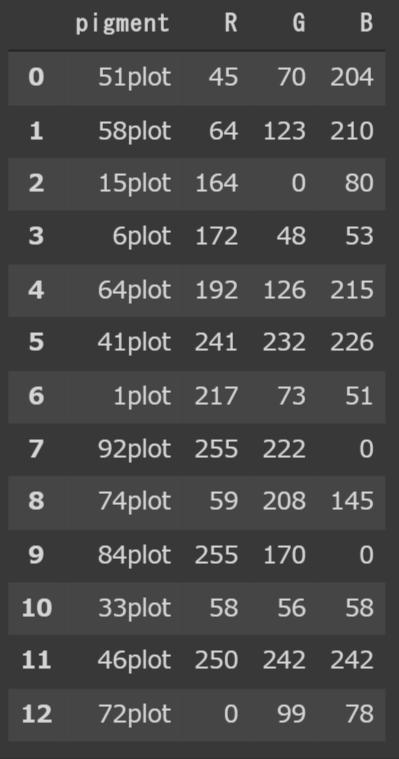
\includegraphics[width=0.34\textwidth]{figures/assignment5/assignment5-sRGB.png}}%
        \hspace*{\fill}
    }
    \caption{Color coordinates in XYZ and sRGB for each pigment}
\end{figure}

\subsection{Brightest and darkest pigments}

According to the definition of the CIEXYZ color system, the $Y$ direction represents luminous intensity response in bright conditions. Since our incident light is D65, we know from Figure \ref{assignment5-xyz} that the brightest and darkest, i.e. having the highest and lowest $Y$ value, are pigment 46 and 33, respectively. We can verify our conclusion by displaying the color directly as shown in Figure \ref{assignment5-sanity-check}.

\begin{figure}[h]
    \centering
    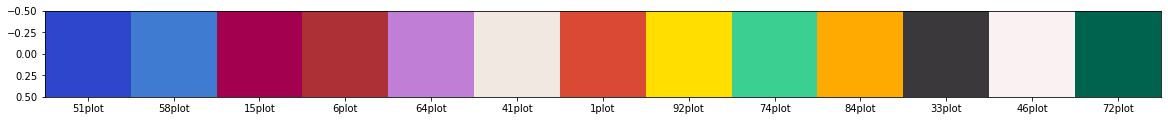
\includegraphics[width=1.0\textwidth]{figures/assignment5/assignment5-sanity-check.png}
    \caption{Color from sRGB coordinates of each pixel}
    \label{assignment5-sanity-check}
\end{figure}

\bibliographystyle{IEEEtran}
\bibliography{citation}

\end{document}